\documentclass[11pt]{article}

% fonts

\usepackage[charter,expert]{mathdesign}
\usepackage{fontspec}
\defaultfontfeatures{Mapping=tex-text}
\setmainfont[Scale=0.95]{CharisSIL}
\setmonofont[Scale=0.8]{Monaco}

% footnote format

\usepackage[hang,ragged]{footmisc}

% pdf with functioning links

\usepackage{ifpdf}
\ifpdf 
    \usepackage[pdftex]{graphicx}   % to include graphics
    \pdfcompresslevel=9 
    \usepackage[pdftex,     % sets up hyperref to use pdftex driver
            plainpages=false,   % allows page i and 1 to exist in the same document
            breaklinks=true,    % link texts can be broken at the end of line
            colorlinks=true,
            hidelinks, % do not show the links with colors or underlining
            pdfauthor={$author-meta$},
            pdftitle={$title-meta$}
           ]{hyperref} 
    \usepackage{thumbpdf}
\else 
    \usepackage{graphicx}       % to include graphics
    \usepackage[hidelinks]{hyperref}       % to simplify the use of \href
\fi 

% bibliography

\usepackage[backend=biber,
            doi=false,
            bibstyle=biblatex-sp-unified,
            citestyle=sp-authoryear-comp
            ]{biblatex}
\addbibresource{/Users/cysouw/Documents/Linguistics/michaellibrary.bib}



\title{Analysing translational survey data through multialignment}
\author{Michael Cysouw \and Jürg Fleischer}
\date{\today}

\begin{document}
  
\maketitle
  
\begin{abstract}
In the analysis of (dialectal) survey data there is a long path of interpretation from the data that is collected to the eventual interpretation. In most past (and current) research there is no paper-trail of all the large and small decisions being taken in the processing of the data. This paper describes as series of methods to document the processing of translational survey data, i.e. data that consists of translational equivalents. As an example we will process 2500 translations of a single sentence from the original Wenker data, transliterated from the original questionnaire from the 19th century. In addition to the well-known geographic distribution of sounds, we will show that it is just as well possible to extract syntactic and lexical variables from this data.
\end{abstract}

\section{Multialigning translations}

There are many ways in which comparable data can be collected to compare different language variants. Possibly the most traditional kind of comparable data (and also often critcized, REF?) are translational equivalent utterances. Language consultants are simply asked to produce the closest possible translation of a given utterance in their language. It is this kind of data that will be the focus of the paper, though the techniques proposed have a much wider application. We will analyse Wenker sentence 9: `\textit{Ich bin bei der Frau gewesen und ich habe es ihr gesagt, und sie sagte, sie wolle es auch ihrer Tochter sagen.}' (I have been at the women and I have told it to her, and she said that she would tell it to her daughter). We have transliterated about 2500 translations from the original Wenker questionnaire, extended with translations from Austria, Switzerland, the Netherlands, Belgium and various german-speaking linguistic enclaves. This data was used at the start of the 20th century to produce the infamous dialectmaps.

\section{Formats for multialignment}

Although one can argue that historical linguistics is from its inception a kind of multialignment, the first explicitly written-down multialignments arose in the context of DNA sequence analysis in biology (cf. Figure~\ref{fig:aminoacids}). In such files each element to be aligned (here amino-acids) are abbreviated with a single character, and the alignment is specified by fixing the position of the characters in a line. Typically, the first ten characters are reserved for a name, and afterwards the characters are just put directly after each other. When an element is missing for one of the species (as so-called `gap'), then a dash `-' is inserted to keep the sequences aligned.

\begin{figure}[htbp] 
	\centering
	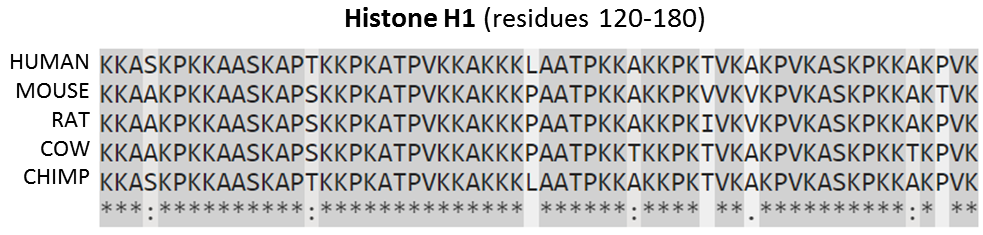
\includegraphics[width=0.8\textwidth]{images/Histone_Alignment.png}
 	\caption{Example of a multiple sequence alignment of amino-acids across biological species.\protect\footnotemark}
	\label{fig:aminoacids}
\end{figure}
\footnotetext{Example from \url{https://en.wikipedia.org/wiki/Sequence_alignment} by T. Shafee.}

This approach can rather straighforwardly be adapted for the multiple alignment of sounds in comparative linguistics. An early example can be seen in Figure~\ref{fig:multialign_bhargava}, aligning various words for `day'. However, one problem with linguistic data is that the assumption of `one element = one letter' is difficult to maintain without strongly simplifying the data. For example, in phonetic transcriptions a single element often consists of multiple Unicode characters, like /aː/ or /t͡ʃ/. In the benchmark data collected by \textcite{list2014benchmark}\footnote{available online at \url{http://alignments.lingpy.org}} they opted to put explicit tab marks between the columns, as illustrated by an example from their database in Figure~\ref{fig:multialign_list}.

\begin{figure}[htbp]
  \centering
  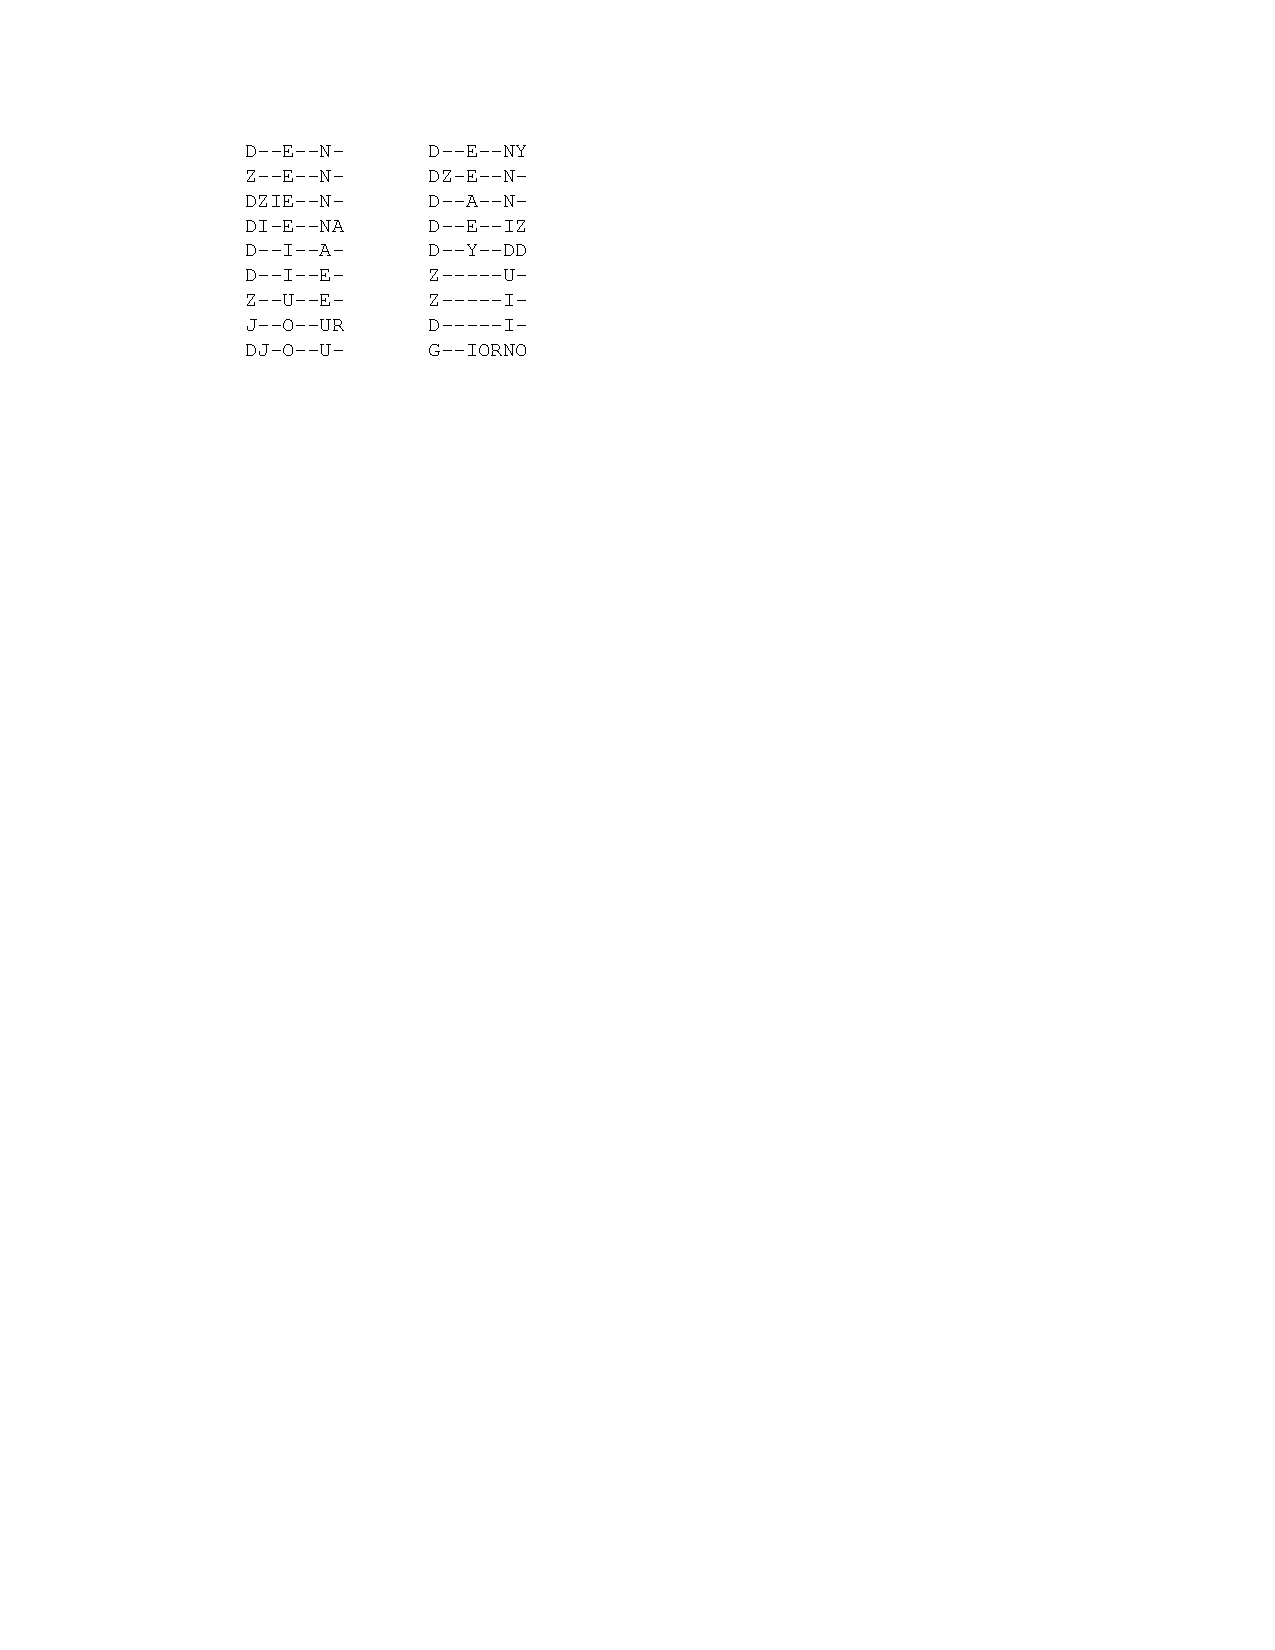
\includegraphics[width=0.5\textwidth]{images/multialign_bhargava.pdf}
  \caption{Linguistic multialignment from \textcite[47]{bhargava2009}.}
  \label{fig:multialign_bhargava}
\end{figure}

\begin{figure}[htbp]
  \centering
  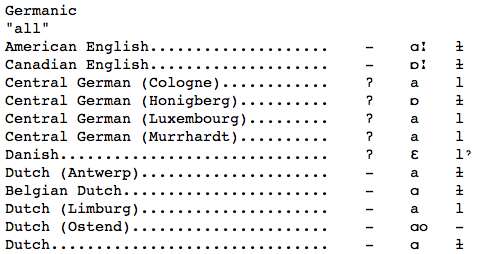
\includegraphics[width=0.8\textwidth]{images/multialign_list.png}
  \caption{Linguistic multialignment with aligned multigraphs and using tabs as separators \parencite{list2014benchmark}}
  \label{fig:multialign_list}
\end{figure}

\printbibliography
\end{document}  
